
\section*{Biographies}

\begin{IEEEbiography}[{
\includegraphics[width=1in,height=1.25in,clip,keepaspectratio]{format/author1.pdf}}]
{Berend J.D. Gort}~was born in Nijmegen, Netherlands, on August 31, 1993. He received his B.Sc. and M.Sc. in mechanical engineering from TU Eindhoven, Netherlands, in 2017 and 2020, respectively, and an M.Sc. in AI \& computer engineering from Harbour.Space, Spain, in 2021. He is currently pursuing a Ph.D. in AI for 6G networking at Universitat Politècnica de Catalunya, Spain. He works as a Full-Stack Machine Learning Engineer at Nearby Computing in Barcelona, Spain, implementing time-series predictions at scale for 6G networks. His previous roles include ML Engineer at Columbia University, where he reduced overfitting in finance models by 46\%, and AI Robotics Engineer at TNO for laser-satellite communications. His research interests include machine learning for time-series forecasting. Gort is a member of IEEE, ACM, and AAAS. He has been awarded the Magna Cum Laude AI \& Computer Science honor.
\end{IEEEbiography}%


\begin{IEEEbiography}[{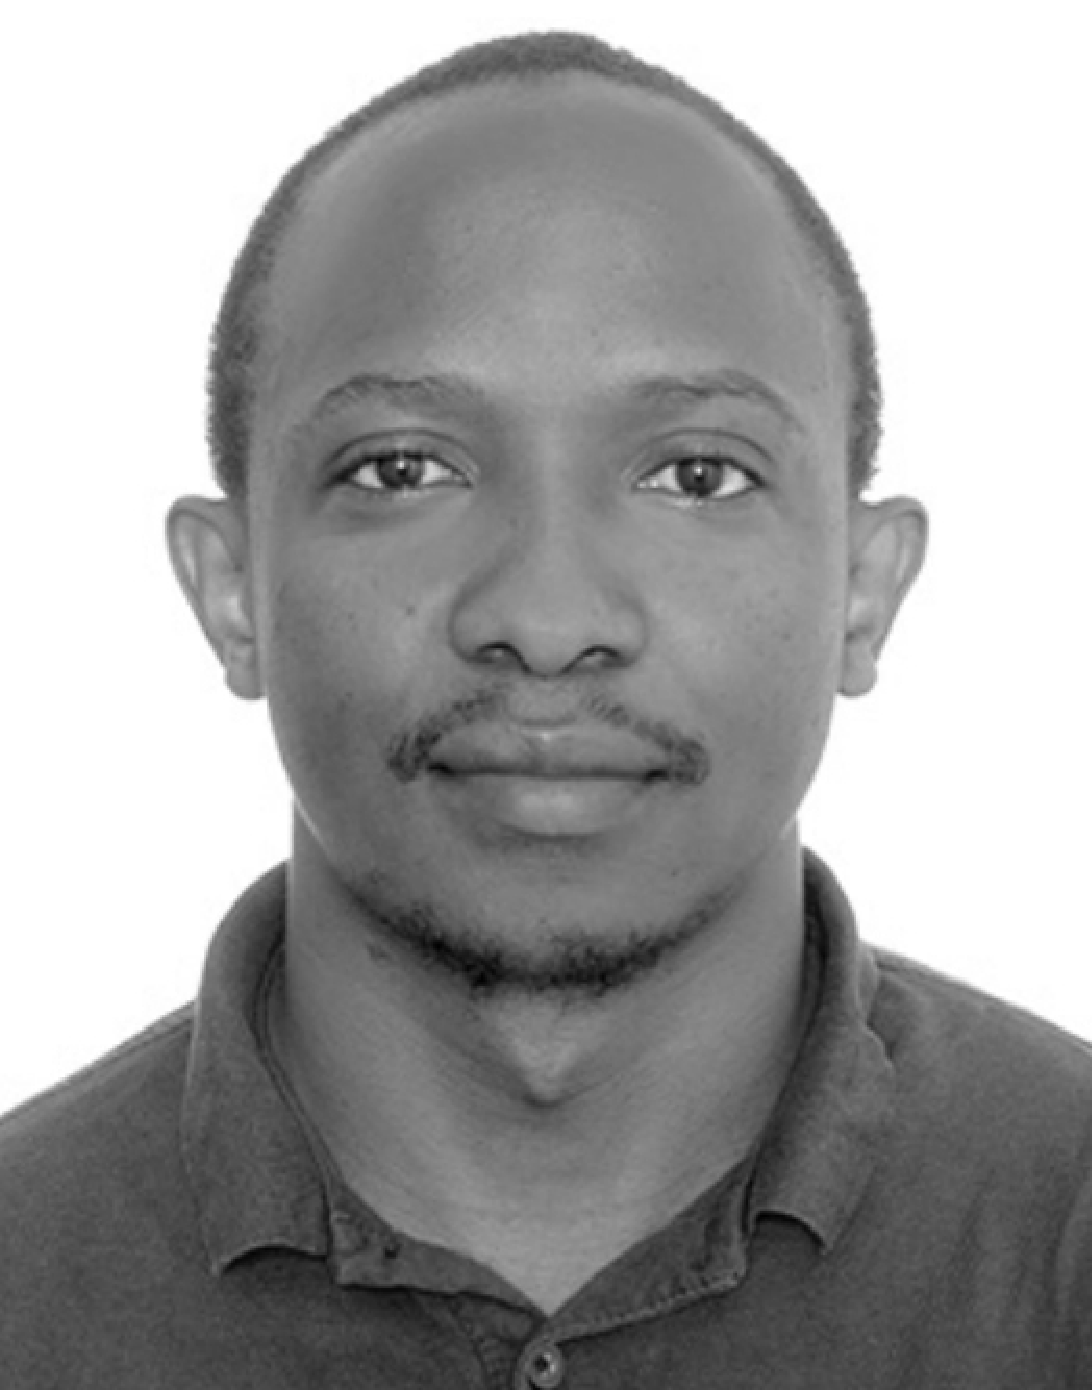
\includegraphics[width=1in,height=1.25in,clip,keepaspectratio]{format/author2.pdf}}]
{Dr. Godfrey M. Kibalya}~received his B.Sc. degree in telecommunications engineering from Makerere University, Uganda, in 2010, his M.Sc. degree in telecommunications engineering from the University of Trento, Italy, and his Ph.D. degree in network engineering from the Technical University of Catalonia (UPC), Spain. He is a Senior Researcher at Nearby Computing and an Assistant Lecturer in the Department of Electrical Engineering at Kabale University, Uganda. His previous experience includes work in telecommunications engineering in Uganda. Dr. Kibalya's research interests focus on network function virtualization and the application of artificial intelligence in network management. He is actively involved in advancing the field of telecommunications through his research and teaching roles.
\end{IEEEbiography}%

\begin{IEEEbiography}
[{
\includegraphics[width=1in,height=1.25in,clip,keepaspectratio]{format/author3.pdf}}]
{Dr. Angelos Antonopoulos}~(Senior Member, IEEE) is currently the Research and Innovation Director
at Nearby Computing S.L. He has authored over 130 papers on various topics, including multi-access edge computing, 5G/6G network architectures, network virtualization/slicing, 5G-ready vertical and over-the-top applications, zero-touch service orchestration, and analytical modeling/optimization in mobile networks.
He has received the Best Paper Award at IEEE GLOBECOM 2014, the Best Demo Award at IEEE CAMAD 2014, and the EURACON Best Paper Award at EuCNC 2016. He has been awarded with the First Prize in the IEEE ComSoc Student Competition (as a Mentor), while he was the Director of the Best UPC Thesis in ICT (2018). He has been on the editorial board of the IEEE Access, IEEE Networking Letters, Computer Networks (Elsevier), and Inventions (MDPI). He has served as officer (Secretary and Vice-Chair) of the IEEE ComSoc Technical Committee on Communication Systems Integration and Modeling (CSIM) and he is an IEEE Senior Member.
\end{IEEEbiography}